\chapter{Introducción y objetivos}

En este primer capítulo, se presenta una introducción al tema principal de la tesis, además de dar un contexto y un marco general del problema que se va a abordar. Asimismo, se establecen los objetivos de la investigación, se describe la estructura general del documento y se enumeran las contribuciones principales que ha generado esta Tesis doctoral.

\section{Introducción}

Esta Tesis se enmarca dentro de las redes definidas por software (\gls{sdn}, por sus siglas en inglés), y las redes programables, las cuales permiten la creación de redes flexibles y adaptables a las necesidades cambiantes de los usuarios y las aplicaciones finales. Este tipo de redes están ganando cada vez más importancia en la sociedad actual, dado que, con la creciente digitalización de la mayoría de los sectores, así como, tejido industrial y social, se están conformando redes cada vez más densas y heterogéneas, que requieren de nuevas tecnologías o herramientas que permitan su gestión y control. La tipología final de estas redes puede ser muy variopinta, pudiendo estar presentes en las redes de comunicaciones, en redes de sensores, en redes de distribución de energía, logística, entre otras.\\
\\
Es por ello, que es difícil acotar el campo de estudio y aplicación de esta Tesis, y no solo por su naturaleza multidisciplinar, sino por la complejidad de que una herramienta o tecnología, sea completamente extrapolable a otro tipo de red. Por ejemplo, se pueden encontrar similitudes entre las necesidades de los distintos tipos de redes, en las redes de comunicaciones móviles \gls{5g} y \gls{6g}, donde existen múltiples dispositivos, sensores y nodos de acceso que deben coordinarse dinámicamente para ofrecer conectividad. En el ámbito energético, donde las redes eléctricas inteligentes o \glspl{sg} destacan por la coordinación dinámica de la integración de fuentes de energía distribuidas, almacenamiento local y consumidores activos. También se puede ver en el campo de la logística, donde se puede considerar el caso de las redes de transporte y distribución, donde los vehículos, almacenes y sistemas de seguimiento deben coordinarse para optimizar rutas, minimizar tiempos de entrega y reducir costes operativos. En todos estos escenarios, el uso de redes programables y softwarizadas ofrecen una base sólida para la gestión flexible y dinámica, sobre la cual se pueden desarrollar herramientas o tecnologías que optimicen cada caso de uso, consiguiendo escenarios más eficientes y adaptables a las necesidades de la red. De ahí que, la idea de esta Tesis sea la de ahondar en las tecnologías habilitantes de las redes programables y definidas por software, y cómo se pueden aplicar en redes densas y con nodos y necesidades heterogéneas. 

\section{Redes programables y definidas por software}

Las redes programables tienen sus raíces en la historia de las redes de comunicación~\cite{meuser2024history}. Desde su inicio, con la llegada de \gls{arpanet} en 1969, creada en Estados Unidos en un contexto de la guerra fría para que los investigadores pudieran intercambiar información, las redes de comunicación han evolucionado desde sistemas simples y estáticos, hacia arquitecturas más complejas y dinámicas. Durante este proceso, la necesidad de controlar y adaptar el comportamiento de la red ha sido un punto recurrente. Sin embargo, durante décadas, las redes tradicionales se caracterizaron por ser muy estáticas, estrechamente ligadas al hardware y al fabricante, lo que dificultaba su evolución y adaptación dinámica a nuevos protocolos o nuevas ideas. Es por ello que, la idea del \gls{sdn} comenzó a gestarse en la Universidad de Stanford en 2003, cuando el profesor asociado de ese entonces, Nick McKeown, planteó las limitaciones de las redes convencionales y la necesidad de replantear cómo operaban los \textit{backbones} \cite{levy2003overhaul}. En 2011, se acuñó el término \gls{sdn}, al mismo tiempo que se lanzó la organización \gls{onf} \cite{onf}, encargada de establecer estándares y promover la difusión del \gls{sdn}, la cual, a finales de 2023 fue incluida en la Linux Foundation para salvaguardar y reafirmar los proyectos y propuestas \textit{open-source} en materia de \textit{Networking}.\\
\\
El paradigma \gls{sdn} \cite{nadeau2013sdn} radica en un concepto de arquitectura de red, en la que, se separa el plano de control (mantenimiento, gestión y control de la red) del plano de datos (lógica de \textit{forwarding}) de la red, para centralizar toda la lógica de control en un único ente, el cual se denomina como controlador. Esta estructura permite lograr una administración de red más centralizada y flexible \cite{nadeau2013sdn}, facilitando la programabilidad de la red y la implementación de herramientas auxiliares que operan directamente sobre la \gls{api} que expone el controlador. Esta \gls{api} de alto nivel es clave en la integración de cualquier tipo de herramienta, desde monitorización, a \gls{qos}, o incluso de modelos de \gls{ai}/\gls{ml} para predecir o reconfigurar la red de forma automática.\\
\\
Este paradigma se empezó a popularizar entre las grandes operadores de telecomunicaciones, que junto a la tecnología de virtualización de funciones de red (del inglés, \gls{nfv})~\cite{etsi2012nfv}, podían desplegar, mantener y gestionar los servicios de red de forma dinámica y escalable, permitiendo al administrador de red operar desde un único de ente de control, toda la infraestructura. Grandes empresas como Google~\cite{vahdat2016purpose}, NTT~\cite{tomonori2013introduction}, IBM~\cite{racherla2014implementing} o Telefónica~\cite{montero2017extending} han contribuido activamente al desarrollo y adopción de estas tecnologías. Este apoyo del sector tecnológico al despliegue de redes \gls{sdn} con \gls{nfv} se ve impulsado por la reutilización de hardware para el despliegue ágil de nuevos servicios y aplicaciones, lo que permite reducir significativamente el gasto en capital (del inglés, \gls{capex}), así como la posibilidad de operar y gestionar la infraestructura de forma centralizada y programable, lo que se traduce en una disminución del gasto operativo (del inglés, \gls{opex}).\\
\\
Sin embargo, las redes softwarizadas y programables no se limitan únicamente a las redes de telecomunicaciones. En los últimos años, se ha podido ver cómo este paradigma se ha extendido a otros campos, como, por ejemplo, en las redes de sensores, donde la flexibilidad y la versatilidad son claves para optimizar el rendimiento de los equipos, que por lo general suelen tener recursos limitados. También se han visto integraciones de ecosistemas \gls{sdn} en el ámbito de las redes de sensores \gls{iot}~\cite{baddeley2018evolving}, donde se provee de una pila de protocolos que permite la interoperabilidad entre los equipos y controladores convencionales, pudiendo traer todos los avances de las redes de telecomunicación a entornos más agresivos, como por ejemplo el \gls{iiot}~\cite{carrascal2025softwarized}.\\
\\
Incluso, se ha llegado a ver el uso de las redes programables en el ámbito de la distribución/encaminamiento de energía, donde la integración de fuentes de energía renovables y la gestión de la demanda dinámica requieren una coordinación meticulosa~\cite{hussain2019optimal}. Históricamente las redes eléctricas de todos los países se han ido conformando en un modelo de top-to-down, donde las grandes centrales eléctricas generaban la energía, y esta se distribuía a los usuarios finales. Con el creciente aumento de la población, la red eléctrica se iba expandiendo y ramificando, creando redes en modo árbol cada vez más densas desde los puntos de interconexión. Sin embargo, con la llegada de las energías renovables y el cambio normativo promovido por la Unión Europea, este modelo tradicional ha comenzado a transformarse. La Directiva 2018/2001/UE sobre energías renovables~\cite{euREDII}, establece un marco regulador que permite a los ciudadanos y empresas convertirse en productores de energía (prosumidores), facilitando no solo el autoconsumo, sino también la posibilidad de inyectar el excedente energético a la red eléctrica. En España, esta directiva se materializó a través del Real Decreto 244/2019~\cite{rd2442019}, que regula el autoconsumo eléctrico y permite compensar económicamente la energía excedentaria. Por lo tanto, se ha pasado a un modelo de red eléctrica, top-to-down, a uno más distribuido y con múltiples puntos de generación, donde los usuarios finales pueden ser tanto consumidores como productores de la energía, haciendo que la red requiera de una mayor flexibilidad y adaptabilidad para gestionar este intercambio de dinamico de energía. Esta necesidad ha llevado a la creación de redes eléctricas inteligentes (\gls{sg}), y a la incorporación de tecnologías de redes programables, que permitan la gestión dinámica de la energía. Estándares como el IEC 61850~\cite{mackiewicz2006overview} han sido claves en el desarrollo para facilitar la interoperabilidad y la comunicación entre diferentes subestaciones y dispositivos dentro de una \gls{sg}, permitiendo integraciones con soluciones \gls{sdn}~\cite{MOLINA2015142,maziku2017software}.\\
\\
De forma similar, las redes de logistica y transporte también han comenzado a adoptar modelos de redes softwarizadas~\cite{hu2015selection}, para optimizar la gestión de flotas, mejorando la eficiencia operativa. Por lo tanto, de forma analoga y sistematica se podría ir sector por sector, viendo como en cada campo de aplicación se van dando redes densas y heterogéneas, que requieren de un enfoque programables, dando lugar a está linea de investigación y desarrollo que se aborda en esta Tesis. A continuación, se presenta el planteamiento del problema y los objetivos de la Tesis, donde se aterriza cómo se va a abordar el estudio de las redes programables y softwarizadas, y en qué campos de aplicación se va a trabajar.


\section{Planteamiento del problema y objetivos de la tesis}

Los objetivos que se plantean en el desarrollo de la Tesis se pueden dividir en dos grandes bloques. Por un lado, se busca profundizar en el estudio de las redes programables, partiendo del escenario base de las redes \gls{sdn}, y con la idea de extender este paradigma a otros campos de aplicación, como son las redes de sensores \gls{iiot} y las redes de distribución de energía. En particular, se busca profundizar en los mecanismos de control empleados en este tipo de redes, los cuales suelen organizarse en torno a dos enfoques principales: el control \textit{out-of-band} y el control \textit{in-band}~\cite{carrascal2023comprehensive}. En el modelo \textit{out-of-band}, cada nodo de red tiene un enlace dedicado con el controlador, permitiendo una separación clara entre el plano de control y el plano de datos. Por el contrario, el modelo \textit{in-band} asume que solo algunos nodos poseen un enlace directo con el controlador, y el resto de los dispositivos reutilizan dicho canal para transmitir información de control.\\
\\
La idea de empezar profundizando este concepto radica en que, después de haber estado trabajando con ello en estudios anteriores, se ha podido ver que, en función del tipo de red y de la topología, uno u otro paradigma puede ser más adecuando, además de no haber una implementación estandarizada en el modelo \textit{in-band}. Esto deja espacio de mejora y optimización tanto para las redes de comunicaciones, como para las redes de sensores y distribución de energía, donde este enfoque puede tener un papel importante. En redes de sensores, por ejemplo, donde los nodos suelen tener capacidades de cómputo, memoria y conectividad limitadas, implementar un enfoque \textit{out-of-band} resulta poco viable. Asimismo, en las redes de distribución eléctrica, en las que la infraestructura sigue habitualmente una topología jerárquica de tipo árbol, no todos los nodos tienen un acceso directo al núcleo de la red, lo que hace necesario explorar soluciones basadas en el control \textit{in-band}. Es por ello, que en el primer bloque de objetivos de la Tesis se busca profundizar en el estudio de mecanismos de control en redes densas y heterogéneas, donde el mecanismo o algoritmo pueda ser adaptado a las necesidades de la red, no solo a encaminamiento sino también a la toma de decisiones de la reconfiguración de la red en aras del intercambio de recursos, como pueda ser capacidad de cómputo, o energía. Además, se contempla el uso de herramientas de \gls{ai}/\gls{ml} como elemento auxiliar en este proceso de control y optimización, con el fin de dotar a la red de capacidades de adaptación proactiva, pudiendo contemplar la predicción de eventos o fallos, y la mejora de las decisiones de reconfiguración y balanceo de carga en tiempo real.\\
\\
Por otro lado, en el segundo bloque de objetivos de la Tesis, se busca analizar en la infraestructura que habilitan las redes softwarizadas, desde un punto de vista de la gestión y en control de la red, así como de la seguridad. En este sentido, se busca profundizar en el uso de herramientas de despliegue, monitorización y gestión de red, que permitan al administrador de red tener una visión global del estado de la infraestructura, así como poder tomar decisiones automáticas sobre la reconfiguración y optimización de la red. Asimismo, se contempla el estudio de las implicaciones de rendimiento que conlleva el uso de redes programables, donde se busca identificar posibles cuellos de botella y proponer soluciones para mitigarlos. En este sentido, se contempla el uso de técnicas de \gls{ai}/\gls{ml} para la reconfiguración de la red, tomando métricas en la comunicación entre los nodos y el controlador. A continuación, en la Figura~\ref{fig:intro_1} se presenta un diagrama general del marco de la Tesis, donde se puede ver cómo se relacionan las distintas áreas de estudio y aplicación, así como los objetivos que se persiguen en cada una de ellas.

\begin{figure}[ht!]
    \centering
    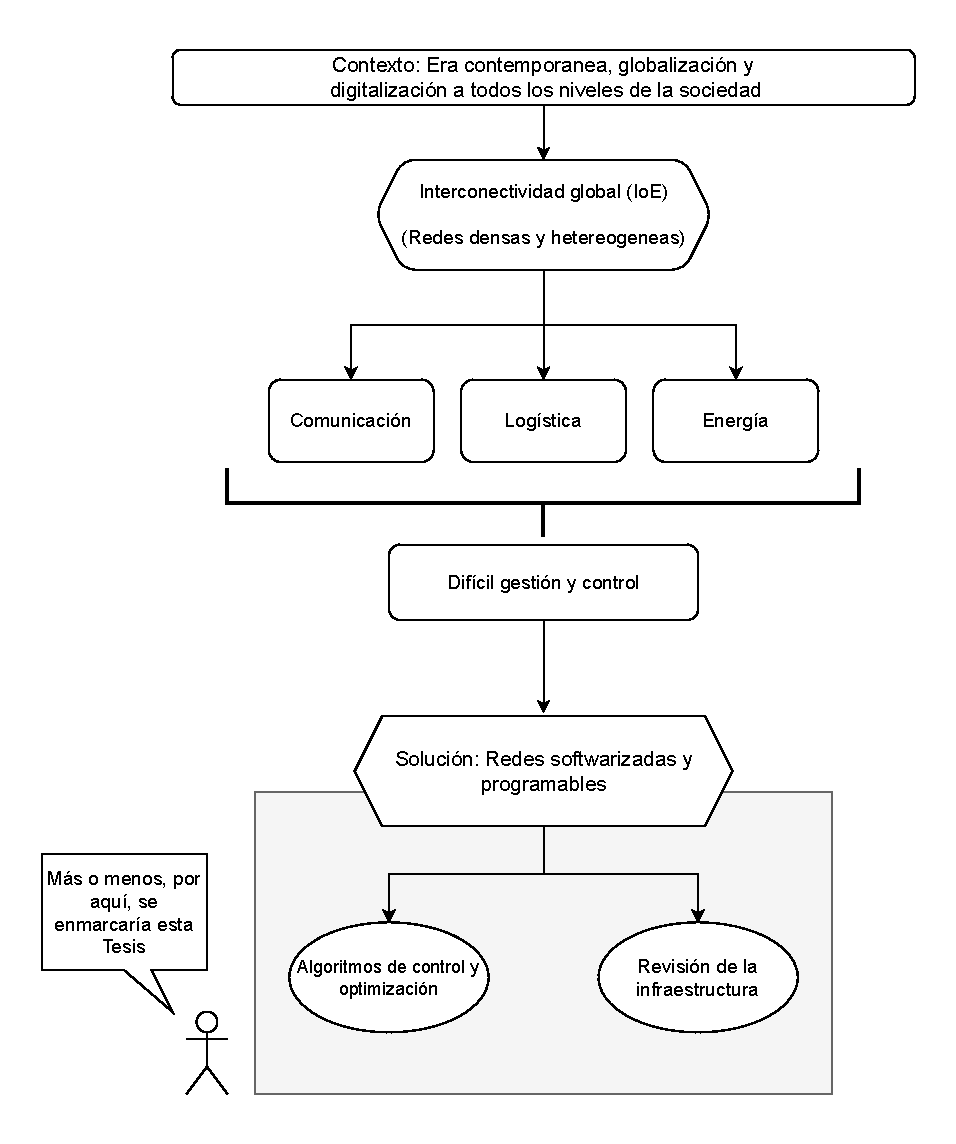
\includegraphics[width=0.85\textwidth]{fig/01_intro/intro_1.drawio.pdf}
    \caption{Diagrama general del marco general de la Tesis}
    \label{fig:intro_1}
\end{figure}

\section{Estructura de la tesis}

A continuación, se presenta la estructura general de esta memoria, describiendo brevemente el contenido de cada uno de sus capítulos. El objetivo es ofrecer una visión global del desarrollo de la Tesis, que sirva como guía para el lector y facilite la comprensión del marco completo del trabajo realizado.\\
\\
El primer capítulo ha contextualizado el ámbito de las redes programables y softwarizadas, destacando su relevancia como base tecnológica para la gestión flexible y dinámica de redes heterogéneas. Asimismo, se ha introducido la problemática asociada a la creciente complejidad de las redes actuales, tanto en las redes de comunicaciones, como las de sensores o las redes de distribución energética, y se han formulado los objetivos principales que guían el desarrollo de esta Tesis. Finalmente, el capítulo concluye con una recopilación de las principales contribuciones científicas generadas a lo largo del trabajo.\\
\\
El segundo capítulo se repasan los conceptos fundamentales y el estado del arte que sustentan la Tesis. El capítulo queda organizado en tres bloques principales. En el primero se abordan las redes programables y softwarizadas, partiendo del paradigma \gls{sdn}, describiendo los modelos de control \textit{out-of-band} e \textit{in-band} y realizando un análisis detallado de las propuestas más relevantes en \textit{in-band}. El segundo bloque se dedica a los servicios y tecnologías habilitadoras en redes softwarizadas y heterogéneas bajo la óptica del MCC (del inglés, Management–Control Continuum): aquí se examinan tanto los servicios básicos (arranque, descubrimiento y provisión de canales de control) como los servicios avanzados (gestión y planificación de recursos, optimización y reconfiguración proactiva de la red). Finalmente, el tercer bloque estudia casos de uso representativos en entornos densos y heterogéneos, con especial atención a las \gls{sg} y a las arquitecturas de sensores \gls{iiot}, para mostrar cómo las tecnologías revisadas se aplican y adaptan a escenarios reales.\\
\\
El tercer capítulo se sintetizan y consolidan los huecos identificados en el capítulo de Estado del Arte, con el objetivo de transformar las lecciones aprendidas en un planteamiento claro del problema, y marcar una hoja de ruta clara para la Tesis.\\
\\
El cuarto capítulo se presenta la primera contribución de la Tesis, una propuesta escalable de control in-band para redes \gls{sdn} orientada a entornos inalámbricos y de baja capacidad, directamente alineada con el primer bloque de objetivos. El capítulo describe en detalle el diseño del protocolo y su implementación práctica (\texttt{win-BOFUSS}), incluyendo los mecanismos de reconocimiento de vecindad, etiquetado jerárquico y mantenimiento de rutas de respaldo. Asimismo, se dedica una sección concreta a la validación experimental en un entorno de emulación inalámbrico, donde se analizan resultados, comportamiento operativo y consideraciones de implementación.\\
\\
El quinto capítulo se presenta DEN2NE, un algoritmo escalable de distribución y reasignación automática de recursos basado en etiquetado jerárquico. El capítulo describe su motivación y principios de diseño, las tres fases principales, la implementación y una evaluación sobre topologías aleatorias que muestra baja complejidad (crecimiento aproximadamente lineal), tiempos de convergencia reducidos y menor señalización en nodos con recursos limitados. DEN2NE contribuye directamente a los objetivos de la Tesis al ofrecer un mecanismo de control y encaminamiento en entornos densos y heterogéneos, y una base para la gestión/planificación de recursos en multitud de casos de uso.\\
\\
El sexto capítulo presenta una propuesta novedosa que integra técnicas de aprendizaje automático (ML) y aprendizaje profundo (DL) para la predicción temprana de fallos en redes inteligentes de distribución eléctrica (SG), apoyada en algoritmos de reconfiguración basados en el etiquetado jerárquico desarrollado en DEN2NE. El capítulo revisa las principales fuentes y conjuntos de datos públicos sobre SG, describe la generación y curación de un nuevo conjunto de datos sobre la ciudad de Funchal (Madeira, Portugal) y detalla cómo se incorporaron perfiles de generación fotovoltaica simulados. A partir de esta base, se entrenan y optimizan diversos modelos ML/DL orientados a operar en entornos densos y heterogéneos, y se dedica un apartado específico a la validación experimental de los modelos, evaluando su capacidad de predicción y su utilidad para guiar reconfiguraciones proactivas de la red.\\
\\
El séptimo capítulo presenta BLOSTE, un algoritmo adaptativo para el encaminamiento de energía en redes de distribución malladas basado en superposiciones lógicas iniciadas desde uno o varios nodos raíz. El capítulo describe su motivación y principios de diseño, los mecanismos de etiquetado y optimización iterativa, la implementación y una evaluación exhaustiva sobre topologías IEEE de referencia y escenarios de gran escala. Los resultados muestran la capacidad de BLOSTE para mantener un balance global de potencia bajo condiciones variables, su escalabilidad (tiempos de convergencia en el orden de milisegundos y crecimiento computacional cercano a lineal), y su robustez frente a topologías y criterios de decisión heterogéneos. BLOSTE contribuye directamente a los objetivos de la Tesis al proporcionar un mecanismo distribuido, flexible y eficiente para la gestión energética en redes malladas, sirviendo como base para el diseño de arquitecturas resilientes en entornos de red complejos.\\
\\
En el capitulo X, .....\\
\\
Por último, el capítulo X recoge las conclusiones principales de la Tesis, así como un bloque que describe futuras líneas de investigación en las que se podrá seguir indagando.


\section{Contribuciones}
\label{sec:contribuciones}
El trabajo desarrollado en esta Tesis Doctoral ha generado una contribución notable a la comunidad científica, tanto en términos de generación de conocimiento como en su difusión y transferencia. En concreto, se han publicado cuatro artículos en revistas indexadas en JCR, incluyendo una publicación en una revista de alto impacto Q1 y tres en Q2, y otra dos más que está en revisión (Q2). Además, se han presentado cuatro trabajos en conferencias internacionales organizadas por el IEEE, lo que demuestra la solidez y el interés internacional del trabajo. Como parte del compromiso con la divulgación científica, los avances de esta Tesis también han sido compartidos en eventos como las X Jornadas de Jóvenes Investigadores de la Universidad de Alcalá y la 5th EUGLOH Annual Student Research Conference 2024. Cabe destacar, como elemento diferenciador, el reconocimiento al potencial de transferencia tecnológica de los resultados de esta investigación, materializado en la obtención del Primer Premio en el Concurso de Ideas para la Creación de Empresas de Base Tecnológica de la UAH en 2024. Este premio pone de relieve la capacidad de esta Tesis no solo para generar conocimiento científico de calidad, sino también para transformarlo en soluciones con impacto real en la sociedad, alineadas con los principios de innovación y transferencia del sistema universitario.\\
\\
Artículos de revista indexadas de alto impacto :

\begin{enumerate}
    \item Carrascal, D., Rojas, E., Arco, J. M., Lopez-Pajares, D., Alvarez-Horcajo, J., \& Carral, J. A. (2023). A comprehensive survey of in-band control in sdn: Challenges and opportunities. Electronics, 12(6), 1265. (JCR Q2)
    
    \item Rojas, E., Carrascal, D., Lopez-Pajares, D., Alvarez-Horcajo, J., Carral, J. A., Arco, J. M., \& Martinez-Yelmo, I. (2024). A Survey on AI-Empowered Softwarized Industrial IoT Networks. Electronics, 13(10), 1979. (JCR Q2)
    
    \item Carrascal, D., Rojas, E., Carral, J. A., Martinez-Yelmo, I., \& Alvarez-Horcajo, J. (2024). Topology-aware scalable resource management in multi-hop dense networks. Heliyon, 10(18). (JCR Q1)
    
    \item Carrascal, D., Bartolomé, P., Rojas, E., Lopez-Pajares, D., Manso, N., \& Diaz-Fuentes, J. (2024). Fault Prediction and Reconfiguration Optimization in Smart Grids: AI-Driven Approach. Future Internet, 16(11), 428. (JCR Q2)
    
    \item Carrascal, D., Santos, C., Rojas, E., Arco, J. M., Lopez-Pajares, D. \& Rodriguez-Sanchez F. J. (2025). Dynamic Energy Routing Using Tree-Based Topologies with Fast Convergence applied to Meshed Microgrids. IEEE Access (under review). (JCR Q2)

    \item Carrascal, D., Díaz-Fuentes, J., Manso, N., Lopez-Pajares, D., Rojas, E., Savi, M. \& Arco, J. M. (2025). Softwarized Edge Intelligence for Advanced IIoT Ecosystems: A Data-Driven Architecture Across the Cloud/Edge Continuum. Applied Sciences (under review). (JCR Q2)
  
\end{enumerate}

Conferencias internacionales:

\begin{enumerate}
    \item Carrascal, D., Rojas, E., Lopez-Pajares, D., Manso, N., \& Gutierrez, E. (2023, December). A scalable SDN in-band control protocol for IoT networks in 6G environments. In 2023 6th International Conference on Advanced Communication Technologies and Networking (CommNet) (pp. 1-7). IEEE.
    
    \item Rojas, E., Carrascal, D., Lopez-Pajares, D., Manso, N., \& Arco, J. M. (2024, February). Towards ai-enabled cloud continuum for iiot: Challenges and opportunities. In 2024 International Conference on Artificial Intelligence, Computer, Data Sciences and Applications (ACDSA) (pp. 1-6). IEEE.
    
    \item Comeron, R., Rojas, E., Carrascal, D., Alvarez-Horcajo, J., \& Arco, J. M. (2024, October). Multi-hop collaborative edge computing involving constrained IoT devices at the far edge. In 2024 15th International Conference on Network of the Future (NoF) (pp. 22-24). IEEE.
 
    \item Carrascal, D., Rojas, E., Lopez-Pajares, D., Manso, N., Alvarez-Horcajo, J., \& Martinez-Yelmo, I. (2025, March). Softwarized Data-Driven Architecture for Edge Computing IIoT Environments: A Proof of Concept. In 2025 28th Conference on Innovation in Clouds, Internet and Networks (ICIN) (pp. 64-68). IEEE.
    
\end{enumerate}

Actvidades de divulgación:

\begin{enumerate}
    \item Ponentes a las X Jornadas de Jóvenes Investigadores de la UAH, presentando el trabajo titulado ``DEN2NE: origen, presente, ¿y futuro?''.
    
    \item Participación en la 5th EUGLOH Annual Student Research Conference 2024, con el trabajo titulado ``Advancements in Enabling Technologies for Programmable and Software-Defined Networks: Paving the Way to 6G''.
\end{enumerate}

Premios:

\begin{enumerate}
    \item Primer Premio - Concurso de ideas para la creación de empresas de base tecnológica - UAH (Programa propio de investigación y transferencia de la UAH 2024).
\end{enumerate}

% \begin{figure}[ht]
% \centering
% \resizebox{\textwidth}{!}{%
% \begin{tikzpicture}[
%   font=\small,
%   node distance=1.2cm,
%   milestone/.style={rectangle, draw, rounded corners, fill=blue!10, text width=6cm, align=left},
%   conf/.style={rectangle, draw, rounded corners, fill=green!20, text width=6cm, align=left},
%   year/.style={circle, draw, fill=black!10, minimum size=1cm},
%   line/.style={-{Stealth}, thick}
% ]

% % Año 2023
% \node[year] (y2023) {2023};
% \node[milestone, below=of y2023] (j1) {Electronics 12(6):\\ In-band control in SDN (JCR Q2)};
% \node[conf, below=of j1] (c1) {CommNet 2023:\\ Scalable in-band protocol for IoT};

% % Año 2024
% \node[year, right=6.5cm of y2023] (y2024) {2024};
% \node[milestone, below=of y2024] (j2) {Electronics 13(10):\\ AI for Softwarized IIoT (JCR Q2)};
% \node[milestone, below=of j2] (j3) {Heliyon 10(18):\\ Topology-aware resource mgmt (JCR Q1)};
% \node[milestone, below=of j3] (j4) {Future Internet 16(11):\\ Smart Grid fault prediction (JCR Q2)};
% \node[conf, below=of j4] (c2) {ACDSA 2024:\\ Cloud continuum for IIoT};
% \node[conf, below=of c2] (c3) {NoF 2024:\\ Multi-hop edge computing};

% % Año 2025
% \node[year, right=6.5cm of y2024] (y2025) {2025};
% \node[milestone, below=of y2025] (j5) {IEEE Access (under review):\\ Dynamic energy routing (JCR Q2)};
% \node[conf, below=of j5] (c4) {ICIN 2025:\\ Data-driven edge architecture};

% % Flechas desde año a nodos
% \draw[line] (y2023.south) -- (j1.north);
% \draw[line] (j1.south) -- (c1.north);

% \draw[line] (y2024.south) -- (j2.north);
% \draw[line] (y2024.south) -- (j3.north);
% \draw[line] (y2024.south) -- (j4.north);
% \draw[line] (y2024.south) -- (c2.north);
% \draw[line] (y2024.south) -- (c3.north);

% \draw[line] (y2025.south) -- (j5.north);
% \draw[line] (y2025.south) -- (c4.north);

% \end{tikzpicture}%
% }
% \caption{Timeline of scientific contributions (2023–2025): journal publications and international conferences.}
% \label{fig:timeline_papers}
% \end{figure}

\begin{figure}[ht]
\centering
\begin{tikzpicture}[
  font=\small,
  % --- Estilos de los Nodos (ajustados para ser más compactos) ---
  milestone/.style={
    rectangle, 
    draw, 
    rounded corners, 
    fill=blue!10, 
    text width=3.2cm, % Ancho reducido
    align=center,     % Centrado para mejor estética
    minimum height=1.5cm
  },
  conf/.style={
    rectangle, 
    draw, 
    rounded corners, 
    fill=green!20, 
    text width=3.2cm, % Ancho reducido
    align=center,     % Centrado
    minimum height=1.5cm
  },
  year/.style={
    circle, 
    draw, 
    thick,
    fill=white, 
    minimum size=1cm
  },
  line/.style={
    -{Stealth[length=2mm]}, 
    thick,
    draw=black!70
  }
]

% ---- EJE PRINCIPAL DE LA LÍNEA DE TIEMPO ----
\draw[very thick, -{Stealth[length=3mm]}] (-0.5,0) -- (14.5,0);

% ---- AÑO 2023 ----
\node[year] (y2023) at (1,0) {2023};
% Nodos con texto simplificado
\node[milestone, above=0.8cm of y2023] (j1) {Electronics\\(JCR Q2)};
\node[conf, below=0.8cm of y2023] (c1) {CommNet 2023};

% ---- AÑO 2024 ----
\node[year] (y2024) at (7,0) {2024};
% Nodos con texto simplificado y espaciado ajustado
\node[milestone, above left=0.6cm and 0.1cm of y2024] (j3) {Heliyon\\(JCR Q1)};
\node[milestone, above right=0.6cm and 0.1cm of y2024] (j2) {Electronics\\(JCR Q2)};
\node[milestone, above=3cm of y2024] (j4) {Future Internet\\(JCR Q2)};

\node[conf, below left=0.6cm and 0.1cm of y2024] (c2) {ACDSA 2024};
\node[conf, below right=0.6cm and 0.1cm of y2024] (c3) {NoF 2024};


% ---- AÑO 2025 ----
\node[year] (y2025) at (13,0) {2025};
% Nodos con texto simplificado
% Dado que hoy es 12 de junio de 2025, el estado "under review" es muy relevante.
\node[milestone, above=0.8cm of y2025] (j5) {IEEE Access \& Applied Sciences\\(JCR Q2)\\ (under review)};
\node[conf, below=0.8cm of y2025] (c4) {ICIN 2025};

% ---- CONEXIONES A LA LÍNEA DE TIEMPO ----
% Conexiones 2023
\draw[line] (y2023) -- (j1.south);
\draw[line] (y2023) -- (c1.north);

% Conexiones 2024
\draw[line] (y2024) -- (j2.south);
\draw[line] (y2024) -- (j3.south);
\draw[line] (y2024.north) .. controls +(0,0.8) and +(0,-0.8) .. (j4.south);
\draw[line] (y2024) -- (c2.north);
\draw[line] (y2024) -- (c3.north);

% Conexiones 2025
\draw[line] (y2025) -- (j5.south);
\draw[line] (y2025) -- (c4.north);


\end{tikzpicture}
\caption{Línea de tiempo de contribuciones científicas (2023–2025): publicaciones en revistas y conferencias internacionales.}
\label{fig:timeline_papers_v3}
\end{figure}